\subsection{Análise Relacionada à Segunda Questão de Pesquisa}

Esta questão busca verificar se a abordagem orientada a serviços melhora a qualidade dos produtos de software desenvolvidos no CPD/UnB, a fim de satisfazer as necessidades dos usuários. 
Para isso, faz-se uma análise qualitativa da capacidade de manutenibilidade do novo sistema \acrshort{SAE} a partir da experiência dos participantes do estudo de caso. 

A análise foi realizada em conformidade com a norma de qualidade NBR ISO/IEC 9126-1~\cite{iso2003iec}. Esta norma recomenda que seja definido um \emph{modelo de qualidade} para uma avaliação. Assim, foi definido um modelo de qualidade com base no \emph{modelo de qualidade externa e interna} referido pela norma, como mostra a Figura~\ref{fig:modelo_qualidade}. 


% Modelo de qualidade proposto
%======================================================================================

\begin{figure}[htb]
\centering
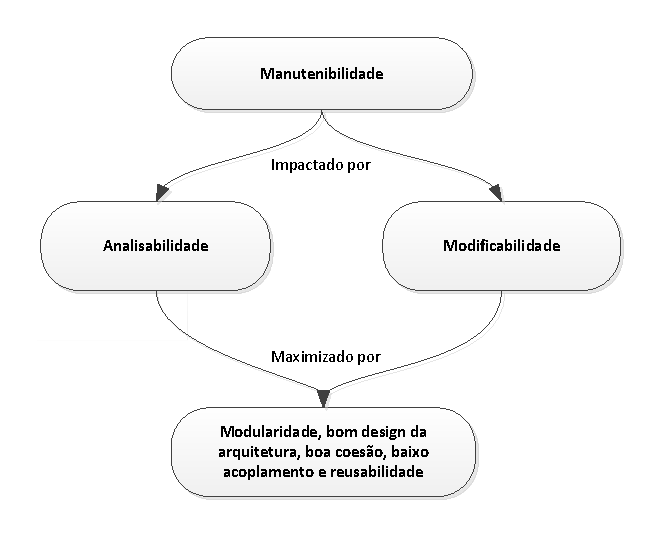
\includegraphics[scale=1]{/img/avaliacao/QP2/modelo_qualidade.pdf}
\caption{Modelo de qualidade proposto para responder a QP2.}
\label{fig:modelo_qualidade}
\end{figure}

O modelo proposto avalia a característica de \emph{manutenibilidade} do
produto de software desenvolvido no estudo de caso (o novo sistema \acrshort{SAE}), 
sendo que foram selecionadas as sub-características da manutenibilidade denominadas
\emph{analisabilidade} e \emph{modificabilidade}, 
as quais servem como uma lista de verificação
de tópicos relacionados com a qualidade avaliada nessa questão. 

A manutenibilidade é uma característica inerente a um produto de software e refere-se a capacidade do mesmo em sofrer correções, melhorias ou adaptações para satisfazerem aos requisitos ou especificações funcionais dos usuários~\cite{iso2003iec, sant2003reuse}. Por definição, a sub-característica analisabilidade compreende a capacidade do produto de software em permitir um diagnóstico das deficiências ou causas de falhas no software, ou a identificação de partes a serem modificadas. Por sua vez, a sub-característica modificabilidade representa a capacidade do produto de software em permitir que uma modificação especificada seja implementada~\cite{iso2003iec}.

É importante salientar, como sugere~\cite{fenton2014software}, que não é possível na prática
medir todas as sub-características internas e externas de um produto
de software, razão pela qual delimitou-se 
nesta investigação as sub-características analisabilidade e modificabilidade
da manutenibilidade, uma vez que o
foco do trabalho de dissertação é propor uma abordagem \acrshort{SOA} 
que seja de fácil manutenção. 

Tradicionalmente, o trabalho de manutenção em um software ocorre após o mesmo entrar em produção e é necessário satisfazer algum requisito ou necessidade que justifique a sua alteração. Para~\cite{S01_bennett2000software}, a manutenção prolonga a vida útil de um software ao mantê-lo atualizado, devendo ser incorporada ao produto de software desde o início de seu desenvolvimento.

Em um primeiro momento, buscou-se verificar a manutenibilidade do sistema \acrshort{SAE}, analisando empiricamente as sub-características analisabilidade e modificabilidade de forma qualitativa. Posteriormente, ao final deste capítulo, será apresentado uma avaliação quantitativa baseada nas métricas propostas por Chidamber \& Kemere~\cite{chidamber1994metrics} para complementar a análise qualitativa, sendo portanto, secundário neste trabalho de dissertação.

De acordo com~\cite{sant2003reuse}, há várias formas de se avaliar a manutenibilidade de um produto de software. Por exemplo, medindo o tempo para aplicar determinada alteração no código fonte ou esforço para diagnosticar determinado problema no software. Também pode-se acompanhar o histórico de modificações de um sistema no repositório de versões desse software. Nesta avaliação, optou-se por mensurar a manutenibilidade por meio da comparação do código fonte do \acrshort{SAE} e outros sistemas da \acrshort{UnB}.

As Figuras~\ref{fig:dependency_diagram_sae_vb},~\ref{fig:dependency_diagram_sae_csharp} 
e~\ref{fig:dependency_diagram_sae_java} mostram três diagramas da arquitetura do \acrshort{SAE} e suas dependências nas versões VB, C\# e Java, respectivamente. Destaca-se que a versão em Java foi desenvolvida durante o estudo de caso com a abordagem proposta neste trabalho de dissertação. Esses diagramas foram produzidos 
utilizando a suíte de ferramentas de análise estática da empresa CodeGear, 
disponível no sítio \url{http://www.codergears.com}. 

Como pode-se observar nos diagramas apresentados, tanto a versão VB quanto a C\# possuem um design monolítico em sua arquitetura. O design monolítico compreende uma das arquiteturas mais comuns e antigas da Engenharia de Software, onde os componentes estão contidos no núcleo do sistema. Nesse \emph{tipo de arquitetura}, como salienta~\cite{clements2002documenting}, a aplicação é composta por vários módulos que são compilados e unidos formando um grande sistema. A maioria dos sistemas em VB e C\# da \acrshort{UnB} segue esta arquitetura, sendo projetados com baixa modularidade e sem qualquer compromisso com o reuso na época em que foram desenvolvidos. 

Segundo o Gestor dos sistemas acadêmicos do CPD/UnB, os principais problemas decorrentes dessa arquitetura, observados nos sistemas legados da \acrshort{UnB}, estão relacionados com a complexidade e o tamanho dos códigos fonte que dificultam a compreensão e a manutenção. Por exemplo, na versão VB do \acrshort{SAE} 
identificou-se um artefato chamado \emph{frmAtzEstSocioEconomico} com aproximadamente 6673 linhas de código. 

Nesse caso, módulos com muitas responsabilidades são difíceis de entender, como é possível presumir, tornando a manutenção muito resistente, passível de erros e comprometendo as propriedades de analisabilidade e modificabilidade. Por conta disso, os desenvolvedores do CPD/UnB, geralmente, evitam alterar os sistemas legados, a não ser quando realmente necessárias.

De modo geral, a única forma de reuso nesses sistemas se dá por meio do acesso ao banco de dados ou através de bibliotecas de funções. Assim, quando necessita-se compartilhar dados ou alguma lógica de negócio, normalmente, criam-se \textit{views} ou \textit{stored procedures} no banco de dados. As bibliotecas de funções contém funções de uso geral e não estão estritamente ligadas as regras de negócios dos sistemas da \acrshort{UnB}. Especificamente, nas aplicações em VB, são muito comuns as regras de negócios estarem na mesma camada onde implementam-se as interfaces com o usuário. Consequentemente, fragmentos de regras de negócios são replicadas em várias telas, dificultando a modificação do software, pois se uma regra mudar, o desenvolvedor precisa revisar o código do sistema para garantir que a lógica foi alterada em todos os locais. 

Por outro lado, até mesmo os sistemas desenvolvidos em Java a partir de 2010
seguem uma arquitetura monolítica com algumas melhorias de design discutidas mais adiante, como 
é o caso do sistema \acrshort{SIGER}, o gerador de relatórios para as aplicações web; o \acrshort{SIEX}, o sistema de informações e extensão; e o \acrshort{SIMAR}, o sistema para gestão das compras de materiais da Universidade. Como curiosidade, o \acrshort{SIMAR} foi migrado parcialmente para Java de acordo com o seu direcionamento estratégico que foi priorizar o módulo de pedidos enquanto que o restante do sistema continuaria funcionando na versão legada. Note que,
sem uma abordagem orientada a serviços, as regras de negócios contidas na versão VB do \acrshort{SIMAR} foram replicadas na versão em Java e, atualmente, a versão Java já contém funcionalidades
não presentes na versão legada, resultado da evolução natural do sistema para atender os 
requisitos dos usuários.


Os sistemas em C\# e Java da \acrshort{UnB} utilizam também uma arquitetura em três camadas para separar a interface com o usuário, o domínio de negócio e a camada de persistência das aplicações. De acordo com a literatura, a arquitetura em camadas auxilia na separação de conceitos e pode trazer ganhos na facilidade de compreensão e na manutenção dos sistemas~\cite{clements2002documenting}. Contudo, o design das aplicações da \acrshort{UnB} continuaram monolíticas, não sendo possível conversarem entre si, a não ser pelo banco de dados. Mesmo com a introdução de bibliotecas compartilhadas para as regras de negócios (introduzido pelo CPD em 2013), ainda era necessário recompilar os sistemas e muitas vezes o desenvolvedor não conseguia reutilizar as bibliotecas devido as dependências circulares existentes. A impossibilidade de reutilizar as regras de negócios de maneira fácil acabou gerando um grande problema para o CPD: a duplicação das classes de negócios entre os sistemas. Assim, os códigos das classes de negócios foram sendo aos poucos replicados entre os sistemas, conforme a necessidade do desenvolvedor. A Figura \ref{fig:duplicidade_usuario_negocio} ilustra esse problema com a classe \emph{UsuarioNegocio} que está replicada em vários sistemas Java. Outro ponto colateral dessas redundâncias, é que muitas classes após serem replicadas, sofrem modificações e começam a evoluir separadamente.

\begin{figure}[ht]
\centering
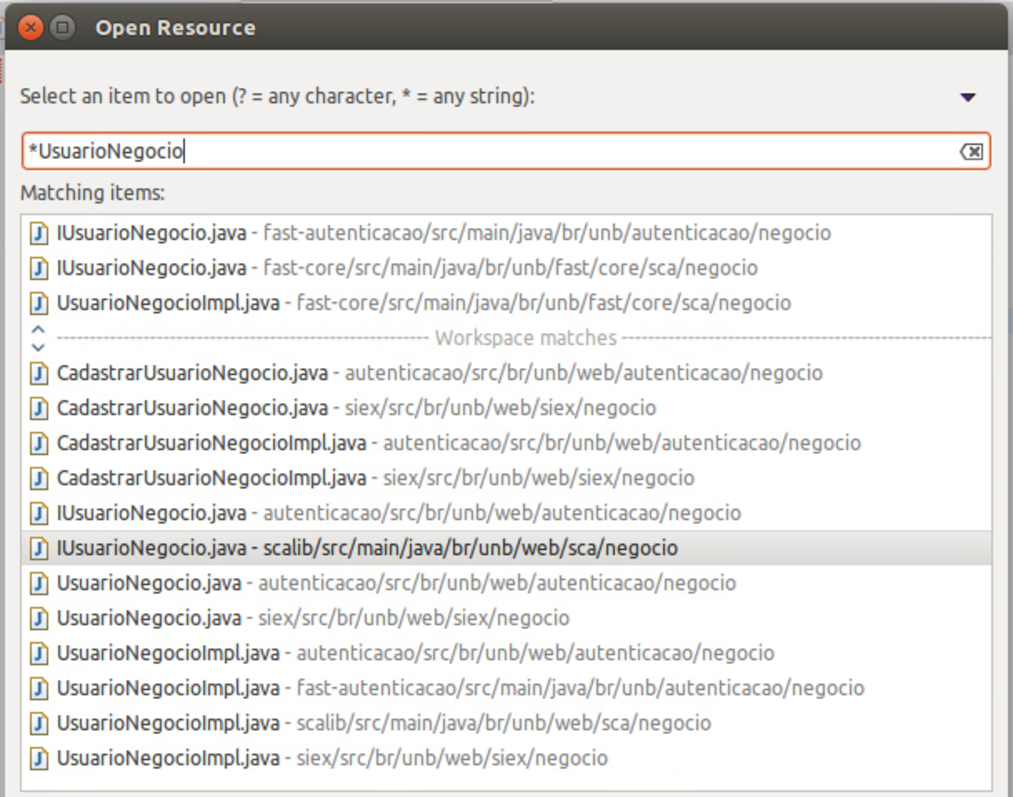
\includegraphics[scale=0.8]{img/avaliacao/QP2/duplicidade_usuario_negocio.pdf}
\caption{Exemplo de classe duplicada entre os sistemas Java.}
\label{fig:duplicidade_usuario_negocio}
\end{figure}

De acordo com o exposto, percebe-se que a manutenibilidade dos sistemas legados da Universidade
(como o \acrshort{SAE} legado) e mesmo os sistemas migrados para Java a partir de 2010,
foram muito impactados pela ausência de modularidade, integração e um bom design arquitetural, tendo como alguns efeitos colaterais observados já discutidos, a duplicidade das regras de negócios, a falta de reuso, a complexidade dos sistemas e o alto custo de manutenção. Assim, possivelmente, uma abordagem SOA aliada a uma boa arquitetura para o desenvolvimento dos serviços poderia minimizar tais problemas.

Nesse aspecto, o último diagrama da Figura~\ref{fig:dependency_diagram_sae_java}, apresenta a arquitetura do novo \acrshort{SAE} usando a arquitetura da abordagem proposta. Uma das preocupações levantadas desde o início dos trabalhos foi a integração lógica das aplicações através de uma camada \acrshort{SOA}, sendo esse papel, realizado pelo barramento e pelo \acrshort{SDK} \emph{ems\_java}, que juntos forneceram uma plataforma \acrshort{SOA} aderente à arquitetura \emph{RESTful} para o projeto. Como é possível notar no diagrama, todos os módulos desenvolvidos na modernização podem compartilhar as suas funcionalidades de forma transparente, bastando invocar os serviços disponíveis no catálogo de serviços do barramento. Salienta-se que o design interno dos módulos auxiliou muito para se chegar nesse objetivo. 

Assim, como discutido na QP1, uma das preocupações dos participantes do estudo de caso foi
empregar um design menos procedimental, razão pela qual decidiu-se utilizar o design \acrshort{DDD}. Este design provê algumas práticas que auxiliam o desenvolvimento de softwares~\cite{evans2004domain}. Uma dessas práticas é a modelagem de domínio do negócio, que promove uma abstração do domínio por meio de um modelo que contempla os aspectos relevantes ao desenvolvimento das aplicações, separando os interesses em domínios de negócios (ou domínios de contextos) separados. Este padrão sugere ainda uma estrutura de objetos que permite que o modelo seja implementado e refletido no código fonte por meio de uma linguagem comum entre as pessoas envolvidas no projeto, seja o especialista no domínio do negócio ou o desenvolvedor~\cite{evans2004domain,vernon2013implementing}. Entre as vantagens indicadas por~\cite{evans2004domain}, está a possibilidade de se obter mais proveito dos benefícios da orientação a objetos, tornando a arquitetura da aplicação mais flexível, fácil de manter e evoluir
com o passar do tempo. 

Nesse sentido, para exemplificar, a Figura~\ref{fig:exemplo_ddd} mostra um exemplo de uma classe Aluno do novo \acrshort{SAE} usando os princípios do \acrshort{DDD}. Foi removido alguns trechos do código fonte original de modo a facilitar a visualização. Como pode-se notar, a classe Aluno possui algumas responsabilidades manifestadas nos métodos declarados nessa classe. Caso fosse utilizado o padrão \textit{Transaction Script}, esta classe não teria nenhum método (objetos anêmicos) e possivelmente as responsabilidades estariam em uma classe de negócio com a classe Aluno servindo meramente como uma estrutura para passar os dados de um aluno entre as camadas do software até a camada de persistência.

\lstset{language=Java,
  basicstyle=\small, %or \small or \footnotesize etc.
  numbersep=10pt,                         % how far the line-numbers are from the code
  tabsize=4,  
  showspaces=false,
  showtabs=false,
  breaklines=true,
  showstringspaces=false,
  breakatwhitespace=true,
  commentstyle=\color{pgreen},
  keywordstyle=\color{pblue},
  stringstyle=\color{pred},
  captionpos=b,
  inputencoding=utf8,
  extendedchars=true,
  literate={á}{{\'a}}1 {ã}{{\~a}}1 {é}{{\'e}}1 {ê}{{\^e}}1 {ç}{{\c{c}}}1 {Ç}{{\c{C}}}1
}
\renewcommand{\lstlistingname}{Código}
\begin{lstlisting}[caption=Exemplo da classe Aluno do sistema SAE, label=fig:exemplo_ddd]
package br.unb.model.sae_context;

public class Aluno {
	private List<OcorrenciaAluno> listaOcorrenciaAluno;

	public void adicionaOcorrenciaAluno(OcorrenciaAluno ocorr){
		if (existeOcorrenciaAberto(ocorr.getSemestreAno(), ocorr.getDataInicio())){
			throw new Exception("O aluno já possui uma ocorrência.");
		}
		
		if (assinouTermoOcorrencia(ocorr.getSemestreAno())){
			throw new Exception("O aluno não possui termo de concessão assinado.");
		}
		
		listaOcorrenciaAluno.add(ocorr);
	}
	
	public List<OcorrenciaAluno> getListaOcorrenciaAluno() {
		return listaOcorrenciaAluno;
	}

	public boolean existeOcorrenciaAberto(String semestreAno, Date dataInicio){
		// Removido para melhor visualização
	}
	
	public boolean assinouTermoOcorrenciaValeAlimentacao(String semestreAno){
		// Removido para melhor visualização
	}
}
\end{lstlisting}





Finalizando a análise da questão QP2, verificaram-se alguns indicativos
qualitativos discutidos que sugerem que a manutenibilidade poderia ser maximizada tanto
pelo processo simplificado da abordagem quanto pela arquitetura
proposta. Porém, alguns desafios identificados durante o estudo de caso
ainda precisam ser melhor investigados para que a abordagem possa ser utilizada. Os 
principais desafios são descritos a seguir:

\begin{itemize}

	\item \textbf{Identificar os serviços que falharam.} A tolerância a falhas não foi o foco deste trabalho mas deverá ser investigado futuramente caso o \acrshort{CPD} opte pela abordagem. Durante os testes, verificou-se que não era possível mapear qual serviço de fato era a origem da falha. Isso pode ser um problema da arquitetura implementada. Por exemplo, quando se introduzia uma falha em um serviço (como o serviço de questionário), vários outros serviços deixavam de funcionar e não era possível identificar que serviço realmente falhou (o que é importante para poder corrigí-lo rapidamente). Seria importante a arquitetura permitir visualizar (se possível) a pilha de chamadas entre os serviços, para verificar qual serviço falhou. Sabe-se que uma das restrições que 
o estilo arquitetural \acrshort{REST} estabelece é que a interação entre 
o cliente e o servidor não deve manter estados entre as comunicações~\cite{fielding2000architectural}. No entanto, a arquitetura da plataforma permite que os serviços comuniquem-se internamente no \textit{cluster} de forma transparente, uma vez que cada serviço é na verdade um processo\footnote{Se o serviço for em Erlang é um processo do ambiente de execução Erlang e, se for em Java é uma \textit{thread} da máquina virtual Java.} que envia/recebe mensagens assíncronas Erlang. Nesse caso, quando um cliente envia uma \emph{requisição REST} para o barramento de serviços e este repassa para o seu destino (o serviço solicitado), a partir daí, as chamadas para outros serviços 
no \textit{cluster} são mensagens Erlang, sendo que nesse caso, poderia haver uma forma de identificar a sequência de chamadas entre os serviços internos para atender a solicitação do cliente, uma vez que todas as chamadas entre os processos passam primeiro pelo processo \emph{Dispatcher} do barramento. 

	\item \textbf{Transformar código procedimental em serviço.}

Este desafio está relacionado as atividades de análise e surgiu devido a dificuldade inerente para transformar código procedural em serviços durante a modernização do \acrshort{SAE}. Note que essa foi uma das atividades identificadas na QP1 mais difíceis de serem realizadas. Em um processo de modernização típico do CPD, que atualmente não é documentado, a migração dos sistemas legados segue o conceito \textit{Transaction Script}, que é relativamente mais direta e fácil de se fazer, uma vez que simplesmente se reescreve o que está no sistema legado para o novo sistema. Não é necessário pensar muito em como fazer, no máximo, vai haver a separação dos códigos de negócios da interface com o usuário e será criado a camada de persistência. Por outro lado, quando se pensa em oferecer serviços reutilizáveis, é necessário pensar na forma como será exposto o serviço, quais os parâmetros de entrada e o que o serviço vai retornar, para que ao final, tenha um bom design da \acrshort{API} e possa ser utilizado pelos clientes.

\end{itemize}


% Diagrama de dependências das três versões do SAE
%======================================================================================


\begin{figure}[htb]
\centering
\includegraphics[scale=0.37]{/img/avaliacao/QP2/metrics/SaeVB/ComponentDependenciesDiagram.png}
\caption{Diagrama de dependências do sistema \acrshort{SAE} na versão VB.}
\label{fig:dependency_diagram_sae_vb}
\end{figure}



\begin{figure}[htb]
\centering
\includegraphics[scale=0.37]{/img/avaliacao/QP2/metrics/SaeWeb/ComponentDependenciesDiagram.png}
\caption{Diagrama de dependências do sistema \acrshort{SAE} na versão C\#.}
\label{fig:dependency_diagram_sae_csharp}
\end{figure}



\begin{figure}[htb]
\centering
\includegraphics[scale=0.4]{/img/avaliacao/QP2/metrics/SaeJava/ComponentDependenciesDiagram.png}
\caption{Diagrama de dependências do sistema \acrshort{SAE} na versão Java.}
\label{fig:dependency_diagram_sae_java}
\end{figure}

